\documentclass[12pt,letterpaper]{article}
\usepackage[papersize={8.5in,11in}]{geometry}
\usepackage{fullpage}
\usepackage{gensymb}
\usepackage[utf8]{inputenc}
\usepackage{graphicx}
\usepackage{amsmath,amsfonts,mathtools,amsthm,subcaption}
\author{Jiaqi Zhu \\Amath 482, Winter 2020}
\title{PCA}

\begin{document}
\maketitle
\begin{abstract}
For this project, we used Principle Componnt Analysis (PCA) to analyze videos of a mass suspended from sping in different ways and understand its behavior of simple physical system based on the idea of Singular Value Decomposition (SVD). Throughout four test trials, the camera may shake or the rotation may be intrdocued, thus resulting some noise data. After all, we will demonstrate various aspect of PCA, its practical usefulness and the effects of noise on the PCA algorithms.
\end{abstract}
\section*{I. Introduction and Overview}
As we mentioned, this project is aimed to illustrate various aspect of PCA, its practical usefulness and the effects of noise on the PCA algorithms. There are four test trails in this project. Three cameras are used to capture the movement of the mass from the spring. The first test is an ideal case which the camera is still and the mass is released straight down, performing a harmonic motion in the z direction. The second test is the noisy case which the mass keeps the same motion as the first test but the camera is shaken to produce some noisy data. The third test is horizontal displacement which the mass is released off-center, performing both a pendulum motion and simple harmonic oscillations in the x-y plane as well as the z direction. The fourth test is horizontal displacement and rotation which the mass is released off-center and rotates. Cameras stay still for the last two tests. Using PCA based on the idea of SVD, we will understand the behavior of each system. 

\section*{II. Theoretical Background}
\subsection*{Singular Value Decomposition (SVD)}
A singular value decomposition (SVD) is a factorization of a matrix into the product of three matrices. In linear algebra, SVD of a matrix A could be written as 
$$A = U\mathbf{\Sigma}V$$
where both U and V are unitary matrices and $\mathbf{\Sigma}$ is a rectangular diagonal matrix. 
\subsection*{Principle Component Analysis (PCA)}
Principle Component Analysis (PCA) is one of the key applications of SVD. Its main purpose is to understand the behaviors of a system by analyzing the data. However, the data may be noisy and redundant for us to analyze. In order to reduce the redundancy, we could consider the covariance between data sets. Consider the two data sets:
$$a = [a_1\:a_2...a_n]\:\:and\:\:b = [b_1\:b_2...b_n]$$
where the variance of a and b are given by
$$\sigma^2_a = \dfrac{1}{n-1}aa^T\: \:and \:\:\sigma^2_b = \dfrac{1}{n-1}bb^T$$
with a covariance between these two data sets 
$$\sigma^2_{ab} = \dfrac{1}{n-1}ab^T$$
where the normalization constant of $1/(n-1)$ is for an unbiased estimator. Suppose matrix X has two sets of data. The appropriate covariance matrix for this case is 
$$C_X = \dfrac{1}{n-1}XX^T$$
whose diagonal represents the variance of particular measurements and the off-diagonal terms are the covariances between measurement types. Large off-diagonal covariance means redundancy and large variance represents the dynamics of interest. Then we should diagonalize the covariance matrix to reduce the redundancy. 
\\SVD is very useful to disgonalize the covariance matrix. We will introduce the transformed variable:
$$Y = U^*X$$
where U is the unitary transformed associated with the SVD: $X = U\mathbf{\Sigma}V^*$, the variance of Y should be 
$$ C_Y = \dfrac{1}{n-1}YY^T = \dfrac{1}{n-1}(U^*X)(U^*X)^T$$
$$ = \dfrac{1}{n-1}U^*(XX^T)U = \dfrac{1}{n-1}U^*U\mathbf{\Sigma}^2UU^* = \dfrac{1}{n-1}\mathbf{\Sigma}^2$$
\section*{III. Algorithm Implementation and Development}
The algorithm for extracting the data and analyze data after PCA is same for the four test trials. For each test, I extracted the data from three cameras respectively and saved the video files to a 4D tensor. Although the video is colored (RGB), we will convert it to grayscale. For each video's first frame, I found a range x and y position (pixel) for the white portion. Then I searched for the maximum of the image data in that range to determine the exact position of the light source. After repeating these steps for each frame, I will have a matrix with two row vectors X and Y for each video, which is totally six data sets for every test. The six vectors' length are not the same because the videos are recorded in different time frame. In order to make this data matrix with same length, we will compute the minimum and truncate the others with the same minumun length. Then we formed a new matrix with 3 matrix with X and Y row vectors and performed SVD on this matrix to obtain the principal components of interest. 
\section*{IV. Computational Results}
\subsection*{Ideal Case}
Note that for the Ideal Case, the mass is released straignt down and the camera keeps still. From Figure 1(a), it's clear to see that there's an oscillation in the y direction but it stays relatively constant in the x direction. From Figure 2(a), we can demonstrate the percentage of variance for the diagonal matrix computed by SVD. We can see that the first value is almost 90 percent, which means that there's only one dominant component, which is just the moving down motion in the z direction. 
\begin{figure}[ht]
\begin{subfigure}{.5\textwidth}
  \centering
  % include first image
  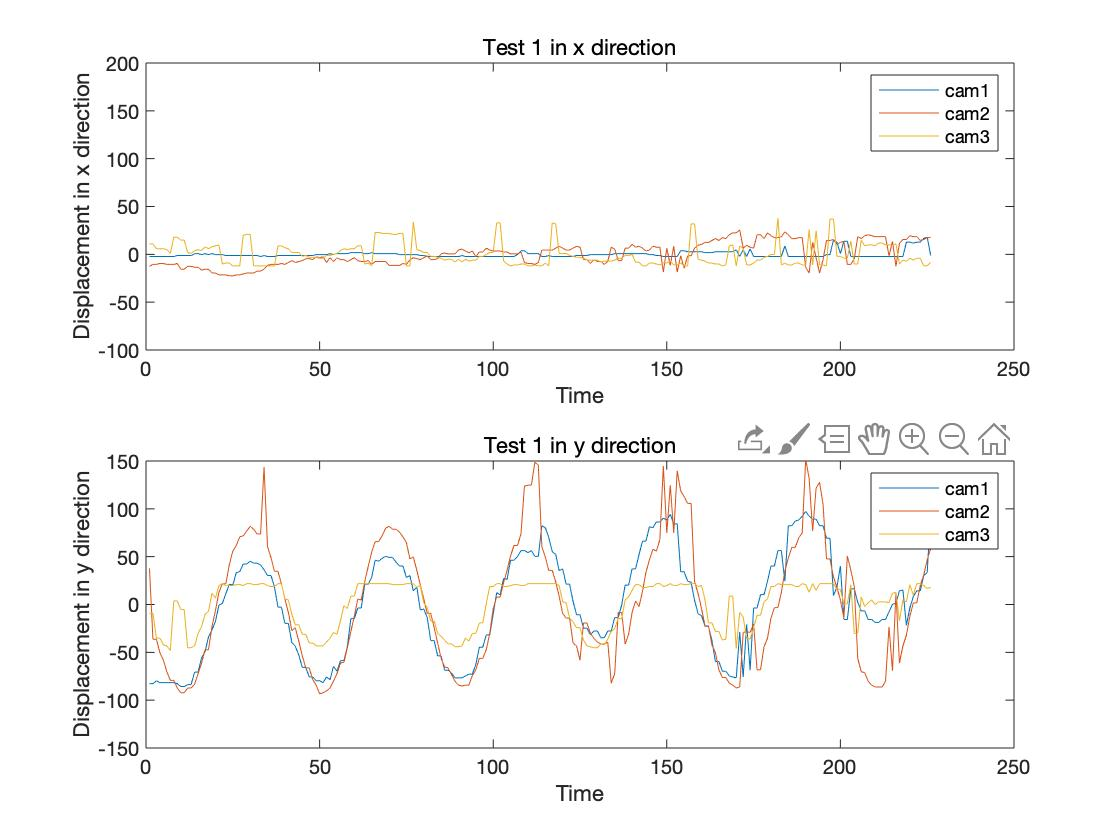
\includegraphics[width=0.9\linewidth]{1-a.jpg}  
  \caption{x and y displacement v.s. time for test 1}
  \label{fig:sub-first}
\end{subfigure}
\begin{subfigure}{.5\textwidth}
  \centering
  % include second image
  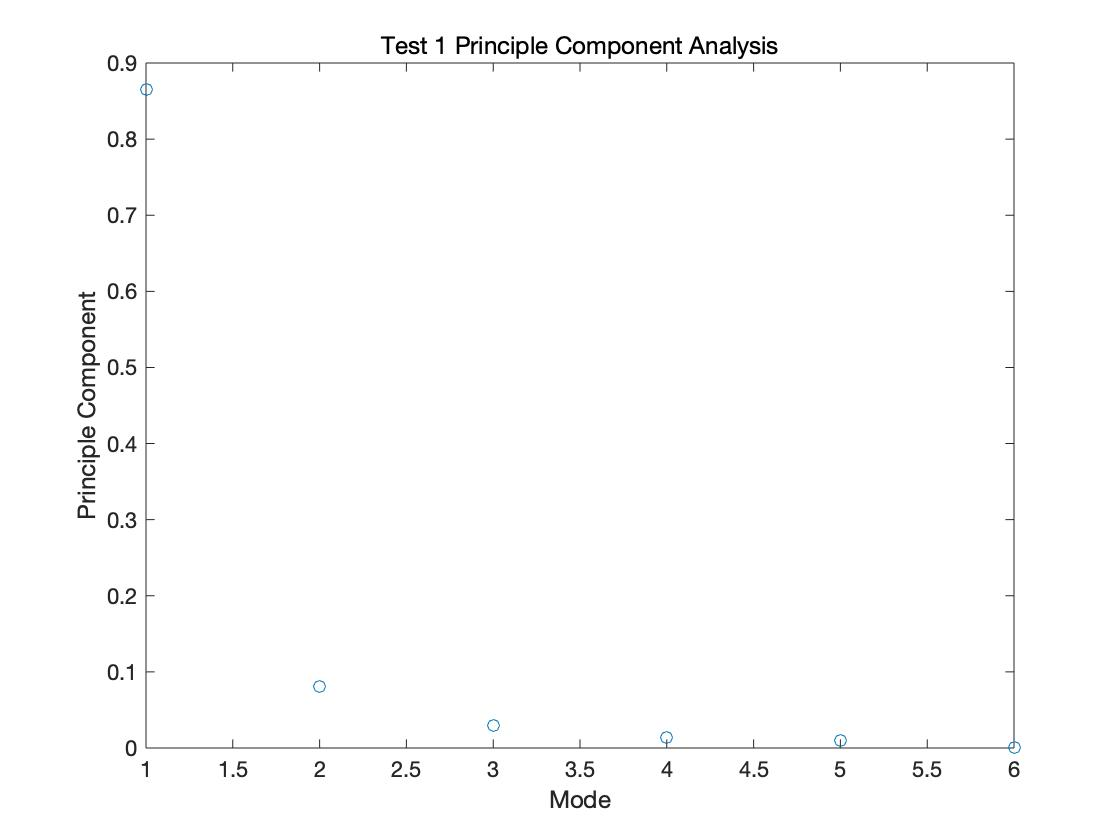
\includegraphics[width=0.9\linewidth]{1-b.jpg}  
  \caption{Principle Component Analysis for test 1}
  \label{fig:sub-second}
\end{subfigure}
\label{fig:fig}
\caption{}
\end{figure}
\subsection*{Noisy Case}
Note that for the noisy case, the mass keeps the same motion as the first case but the camera is shaking, which creates lots of noise data. Because of the shaking camera, we can see that from Figure 2(a), it's hard to extract clear data to form a clear movement of motion in both x and y direction, but we can slightly see the pattern. From Figure 2(b), we can see that the first value is almost 65 percent, which means that there's still a dominant component, even if it weighed less than the first case. We can conclude that there's still only one direction, z direction matters the system. 
\begin{figure}[ht]
\begin{subfigure}{.5\textwidth}
  \centering
  % include first image
  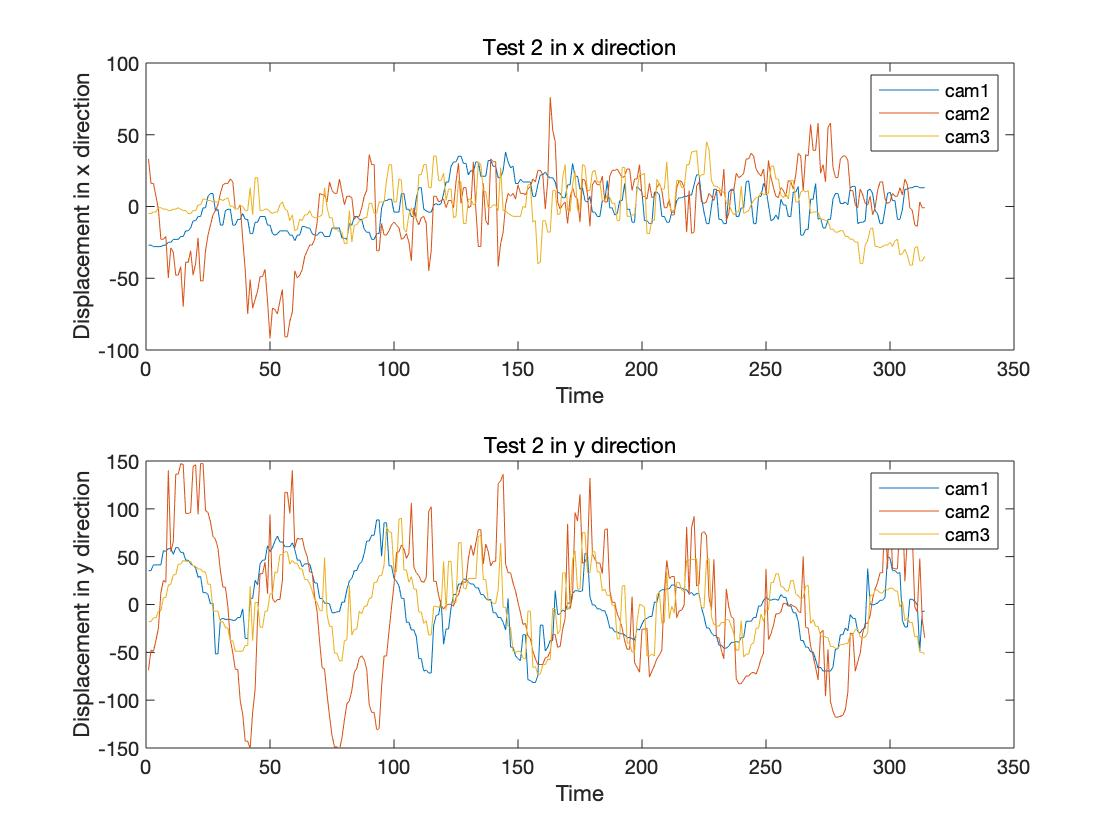
\includegraphics[width=0.9\linewidth]{2-a.jpg}  
  \caption{x and y displacement v.s. time for test 2}
  \label{fig:sub-first}
\end{subfigure}
\begin{subfigure}{.5\textwidth}
  \centering
  % include second image
  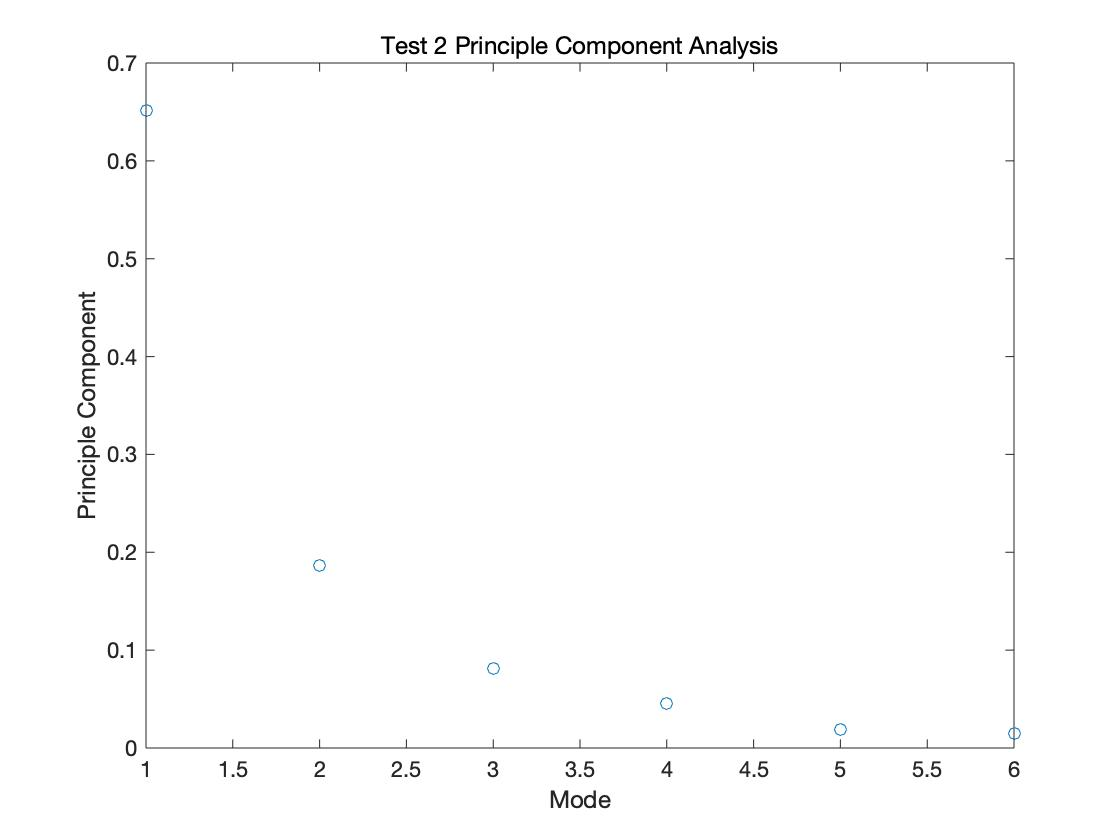
\includegraphics[width=0.9\linewidth]{2-b.jpg}  
  \caption{Principle Component Analysis for test 2}
  \label{fig:sub-second}
\end{subfigure}
\label{fig:fig}
\caption{}
\end{figure}
\subsection*{Horizontal Displacement}
Note that for the horizontal displacement, the mass is released off-center, performing both a pendulum motion and simple harmonic oscillations both in the x - y plane as well as in the z direction.From Figure 3(a), we can see that unlike the first and second case, there's not only a y displacement, there's also one in the x direction.  From the Figure 3(b), we can see that the first and second value is larger than the others, then there're two dominant components in this case. 
\begin{figure}[ht]
\begin{subfigure}{.5\textwidth}
  \centering
  % include first image
  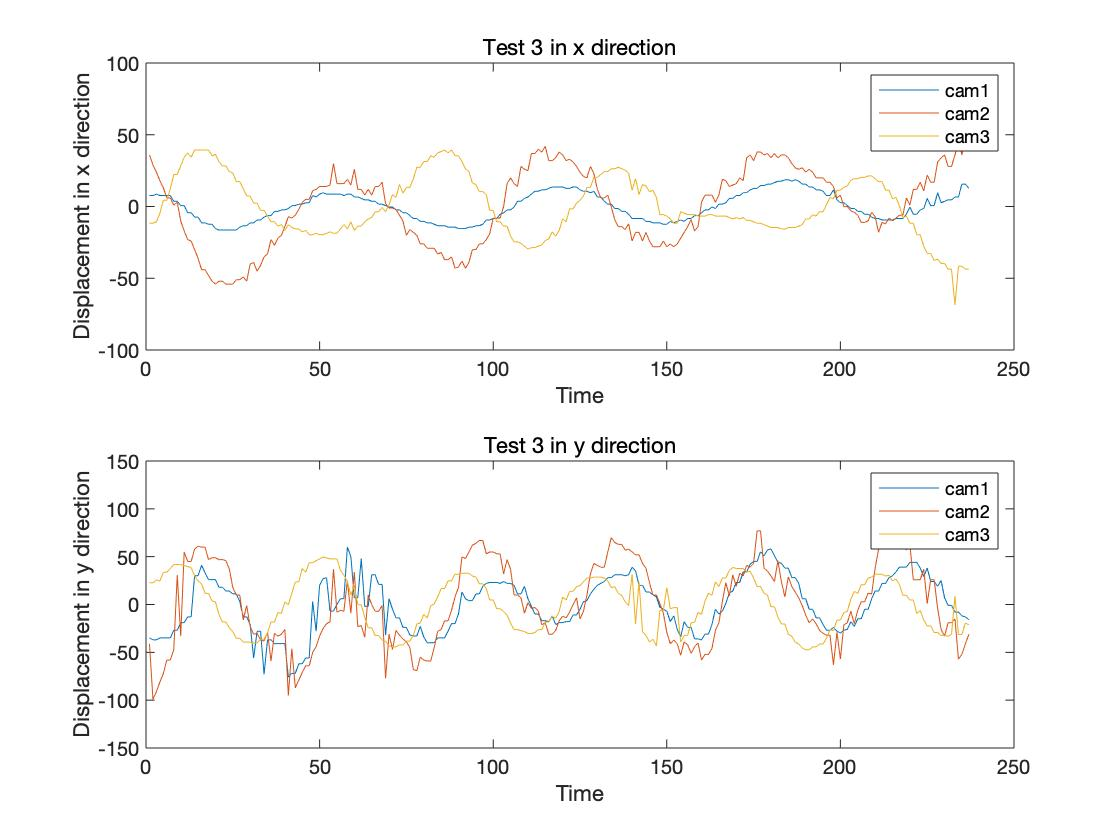
\includegraphics[width=0.9\linewidth]{3-a.jpg}  
  \caption{x and y displacement v.s. time for test 3}
  \label{fig:sub-first}
\end{subfigure}
\begin{subfigure}{.5\textwidth}
  \centering
  % include second image
  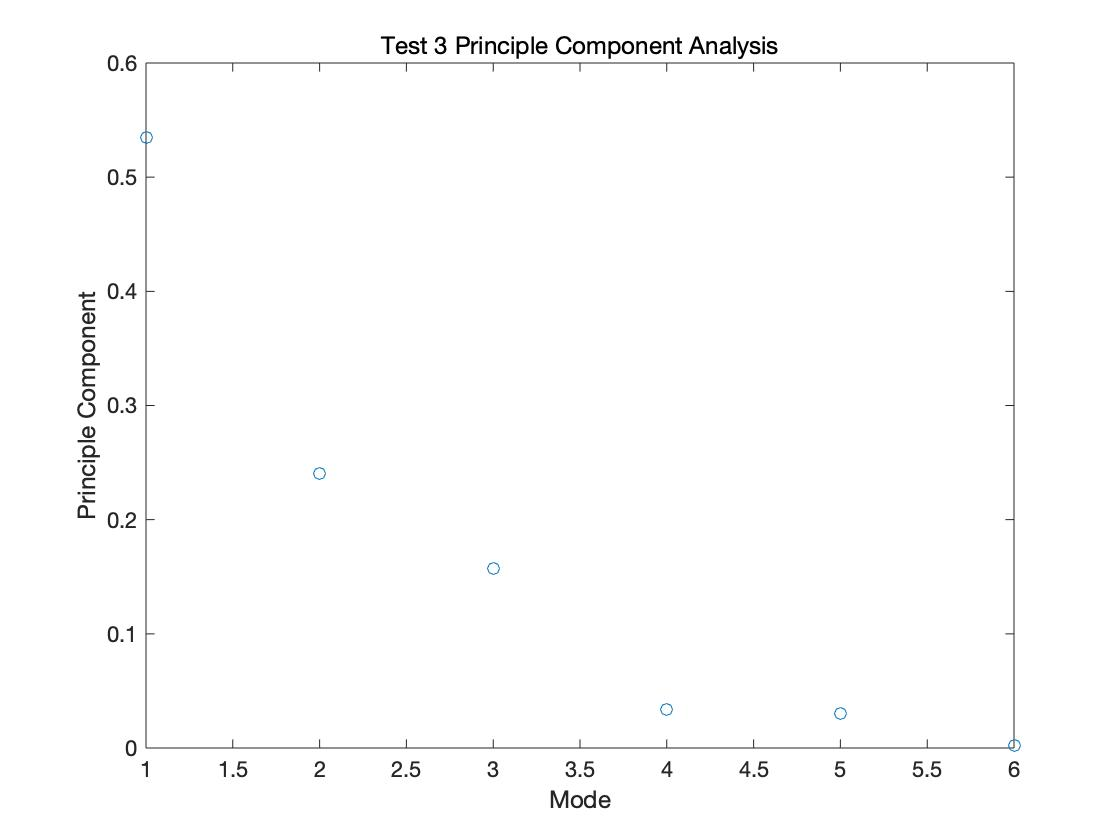
\includegraphics[width=0.9\linewidth]{3-b.jpg}  
  \caption{Principle Component Analysis for test 3}
  \label{fig:sub-second}
\end{subfigure}
\label{fig:fig}
\caption{}
\end{figure}
\subsection*{Horizontal Displacement and Rotation}
Note that for the horizontal displacement, the mass is released off-center and rotates to perform both a pendulum motion in the x - y plane as well as rotation and motion in the z direction. From Figure 4(a), we can see that there's still both x and y displacements. From Figure 4(b), at first glance we may assume that there're only two dominant components; however, compared with Figure 1(b) and Figure 2(b), we can see that the first value is less than that in those figures but others are larger, then there should be three dominant components in this case even though the other two isn' t weighed as much as the first dominant component. 
\begin{figure}[ht]
\begin{subfigure}{.5\textwidth}
  \centering
  % include first image
  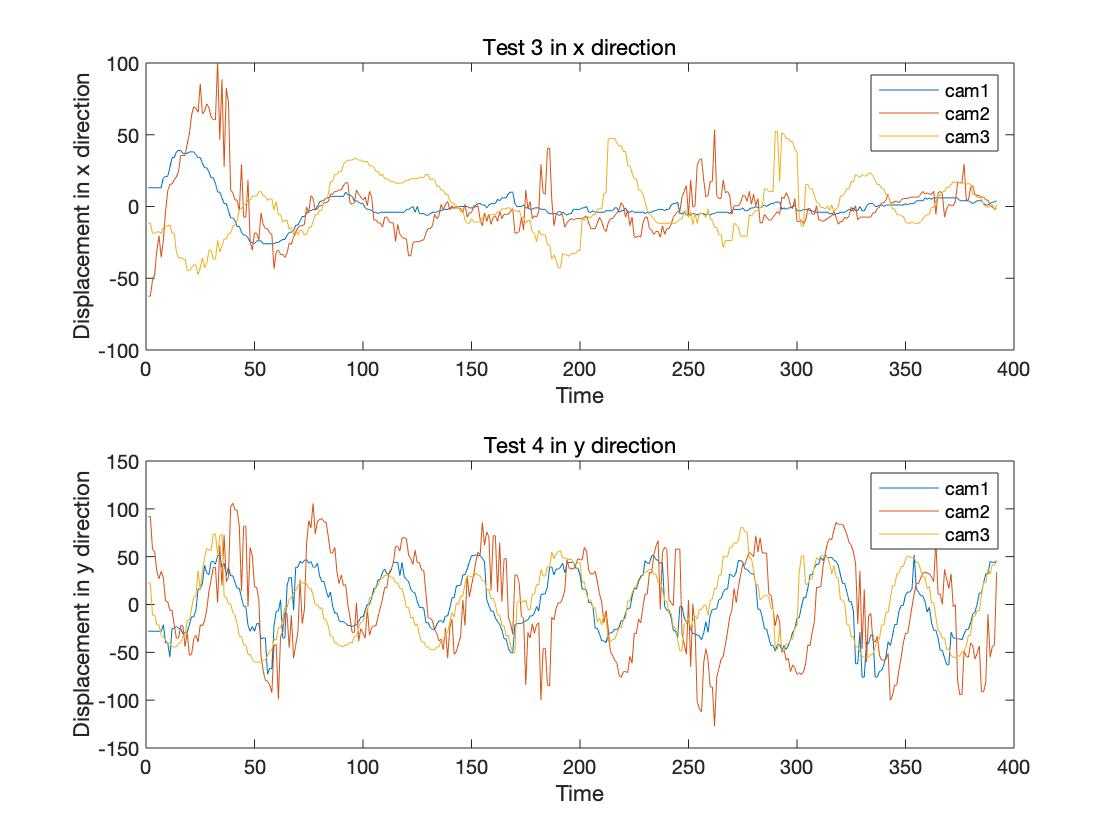
\includegraphics[width=0.9\linewidth]{4-a.jpg}  
  \caption{x and y displacement v.s. time for test 4}
  \label{fig:sub-first}
\end{subfigure}
\begin{subfigure}{.5\textwidth}
  \centering
  % include second image
  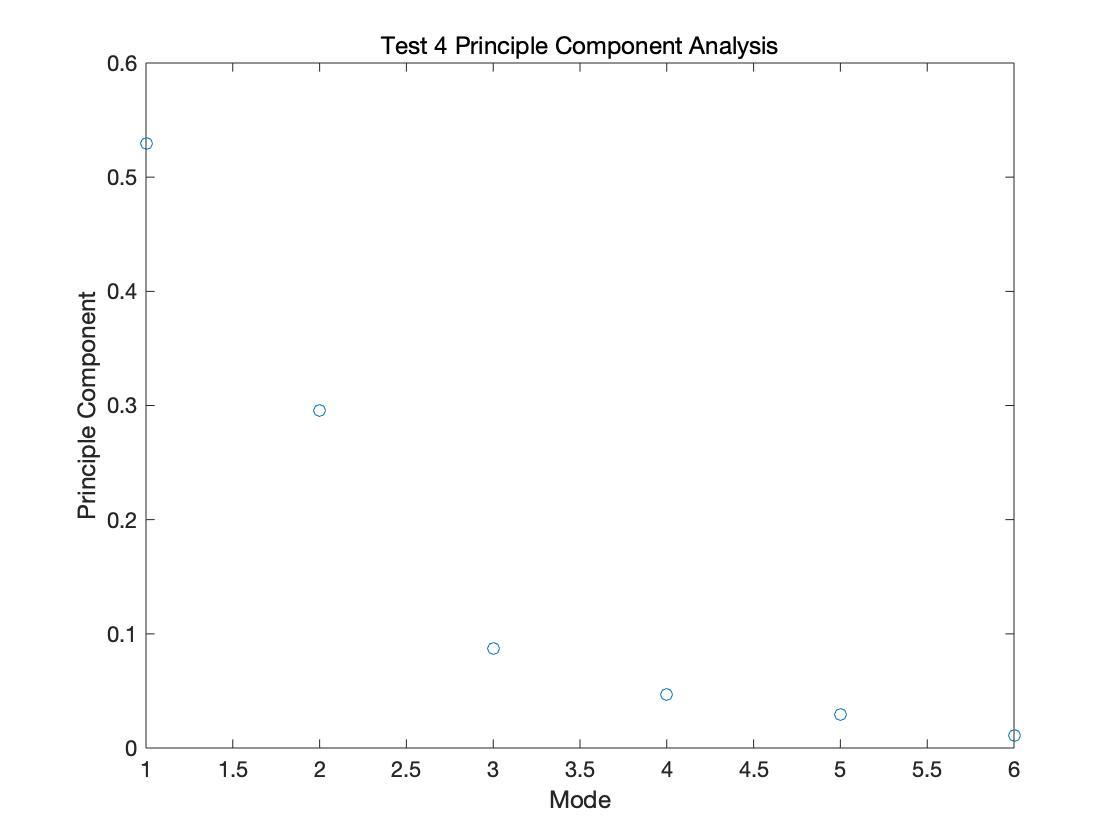
\includegraphics[width=0.9\linewidth]{4-b.jpg}  
  \caption{Principle Component Analysis for test 4}
  \label{fig:sub-second}
\end{subfigure}
\label{fig:fig}
\caption{}
\end{figure}
\section*{V. Summary and Conclusions}
For this project, I applied PCA to analyze and understand the behavior of a simple physical system, which the mass is released from the spring in different ways. For each test trial, we extracted data from videos taken by three different cameras. Based on the idea of SVD, we remove the redundancy of data, determine the max variances,and demonstrate the dominant component in the system. PCA is really powerful to understand the behavior of one system through data analysis based on the idea of SVD. 
\newpage
\section*{Appendix A. MATLAB functions used and brief implementation explanation}
rgb2gray: img = rgb2gray(vidFrames1\_1(:,:,:,i)): convert RGB colored image to grayscale.
\\
\\double: X1 = double(img(:,320:380)): transform the data from unit8 to double precision. 
\\
\\X1(:): convert the matric X1 into a column vector. 
\\
\\mn = mean(X,2): return the mean according to the dimension. Note that X is a matrix with 2 dimension, then it will return a column vector of the mean of each row. 
\\
\\repmat: X = X - repmat(mn,1,n): specifies a list of scalars, 1 and n describes how copies of mn are arranged in each dimension. 
\\
\\svd: [u,s,v]=svd(X'/sqrt(n-1)): performs a singular value decomposition of matrix X'/sqrt(n-1). 
\newpage
\section*{Appendix B. MATLAB codes}
\begin{verbatim}
clear; close all; clc; 
%% test 1
load('cam1_1.mat');
load('cam2_1.mat');
load('cam3_1.mat');

[xlength1, ylength1,a1,num_f1] = size(vidFrames1_1);
data1 = zeros(2,num_f1);
for i = 1:num_f1
    img = rgb2gray(vidFrames1_1(:,:,:,i));
    X1 = double(img(:,320:380));
    [V,I] = max(X1(:));
    [newy,newx] = ind2sub(size(X1),I);
    data1(:,i) = [newx;newy];
end


[xlength2,ylength2,a2,num_f2] = size(vidFrames2_1);
data2 = zeros(2,num_f2);
for i = 1:num_f2
    img = rgb2gray(vidFrames2_1(:,:,:,i));
    X2 = double(img(:,260:340));
    [V,I] = max(X2(:));
    [newy,newx] = ind2sub(size(X2),I);
    data2(:,i) = [newx;newy];
end

[xlength3,ylength3,a3,num_f3] = size(vidFrames3_1);
data3 = zeros(2,num_f3);
for i = 1:num_f3
    img = rgb2gray(vidFrames3_1(:,:,:,i));
    X3 = double(img(250:310,290:360));
    [V,I] = max(X3(:));
    [newy,newx] = ind2sub(size(X3),I);
    data3(:,i) = [newx;newy];
end

minLength = 226;
data1 = data1(:,1:minLength);
data2 = data2(:,10:minLength+9);
data3 = data3(:,1:minLength);

figure(1)
subplot(2,1,1);
plot(data1(1,:)-mean(data1(1,:))), hold on
plot(data2(1,:)-mean(data2(1,:)))
plot(data3(2,:)-mean(data3(2,:)))
xlabel('Time')
ylabel('Displacement in x direction')
ylim([-100, 200])
title('Test 1 in x direction')
legend('cam1','cam2','cam3');
subplot(2,1,2);
plot(data1(2,:)-mean(data1(2,:))), hold on
plot(data2(2,:)-mean(data2(2,:)))
plot(data3(1,:)-mean(data3(1,:)))
xlabel('Time')
ylabel('Displacement in y direction')
ylim([-150, 150])
title('Test 1 in y direction')
legend('cam1','cam2','cam3');
hold off


X = [data1;data2;data3];
[m,n] = size(X);
mn = mean(X,2);
X = X - repmat(mn,1,n);
[u,s,v]=svd(X'/sqrt(n-1));
lambda=diag(s).^2;
figure(2)
plot(lambda/sum(lambda),'o');
xlabel('Mode')
ylabel('Principle Component')
title('Test 1 Principle Component Analysis')

%% test 2
load('cam1_2.mat');
load('cam2_2.mat');
load('cam3_2.mat');

[xlength1, ylength1,a1,num_f1] = size(vidFrames1_2);
data1 = zeros(2,num_f1);
for i = 1:num_f1
    img = rgb2gray(vidFrames1_2(:,:,:,i));
    X1 = double(img(200:400,300:400));
    [V,I] = max(X1(:));
    [newy,newx] = ind2sub(size(X1),I);
    data1(:,i) = [newx;newy];
end


[xlength2,ylength2,a2,num_f2] = size(vidFrames2_2);
data2 = zeros(2,num_f2);
for i = 1:num_f2
    img = rgb2gray(vidFrames2_2(:,:,:,i));
    X2 = double(img(50:370,200:400));
    [V,I] = max(X2(:));
    [newy,newx] = ind2sub(size(X2),I);
    data2(:,i) = [newx;newy];
end

[xlength3,ylength3,a3,num_f3] = size(vidFrames3_2);
data3 = zeros(2,num_f3);
for i = 1:num_f3
    img = rgb2gray(vidFrames3_2(:,:,:,i));
    X3 = double(img(180:320,250:460));
    [V,I] = max(X3(:));
    [newy,newx] = ind2sub(size(X3),I);
    data3(:,i) = [newx;newy];
end

minLength = 314;
data1 = data1(:,1:minLength);
data2 = data2(:,20:minLength+19);
data3 = data3(:,1:minLength);

figure(1)
subplot(2,1,1);
plot(data1(1,:)-mean(data1(1,:))), hold on
plot(data2(1,:)-mean(data2(1,:)))
plot(data3(2,:)-mean(data3(2,:)))
xlabel('Time')
ylabel('Displacement in x direction')
ylim([-100, 100])
title('Test 2 in x direction')
legend('cam1','cam2','cam3');
subplot(2,1,2);
plot(data1(2,:)-mean(data1(2,:))), hold on
plot(data2(2,:)-mean(data2(2,:)))
plot(data3(1,:)-mean(data3(1,:)))
xlabel('Time')
ylabel('Displacement in y direction')
ylim([-150, 150])
title('Test 2 in y direction')
legend('cam1','cam2','cam3');
hold off


X = [data1;data2;data3];
[m,n] = size(X);
mn = mean(X,2);
X = X - repmat(mn,1,n);
[u,s,v]=svd(X'/sqrt(n-1));
lambda=diag(s).^2;
figure(2)
plot(lambda/sum(lambda),'o');
xlabel('Mode')
ylabel('Principle Component')
title('Test 2 Principle Component Analysis')

%% test 3
load('cam1_3.mat');
load('cam2_3.mat');
load('cam3_3.mat');

[xlength1, ylength1,a1,num_f1] = size(vidFrames1_3);
data1 = zeros(2,num_f1);
for i = 1:num_f1
    img = rgb2gray(vidFrames1_3(:,:,:,i));
    X1 = double(img(250:400,200:400));
    [V,I] = max(X1(:));
    [newy,newx] = ind2sub(size(X1),I);
    data1(:,i) = [newx;newy];
end


[xlength2,ylength2,a2,num_f2] = size(vidFrames2_3);
data2 = zeros(2,num_f2);


for i = 1:num_f2
    img = rgb2gray(vidFrames2_3(:,:,:,i));
    X2 = double(img(200:400,220:380));
    [V,I] = max(X2(:));
    [newy,newx] = ind2sub(size(X2),I);
    data2(:,i) = [newx;newy];
end

[xlength3,ylength3,a3,num_f3] = size(vidFrames3_3);
data3 = zeros(2,num_f3);
for i = 1:num_f3
    img = rgb2gray(vidFrames3_3(:,:,:,i));
    X3 = double(img(180:350,150:480));
    [V,I] = max(X3(:));
    [newy,newx] = ind2sub(size(X3),I);
    data3(:,i) = [newx;newy];
end

minLength = 237;
data1 = data1(:,1:minLength);
data2 = data2(:,30:minLength+29);
data3 = data3(:,1:minLength);

figure(1)
subplot(2,1,1);
plot(data1(1,:)-mean(data1(1,:))), hold on
plot(data2(1,:)-mean(data2(1,:)))
plot(data3(2,:)-mean(data3(2,:)))
xlabel('Time')
ylabel('Displacement in x direction')
ylim([-100, 100])
title('Test 3 in x direction')
legend('cam1','cam2','cam3');
subplot(2,1,2);
plot(data1(2,:)-mean(data1(2,:))), hold on
plot(data2(2,:)-mean(data2(2,:)))
plot(data3(1,:)-mean(data3(1,:)))
xlabel('Time')
ylabel('Displacement in y direction')
ylim([-150, 150])
title('Test 3 in y direction')
legend('cam1','cam2','cam3');
hold off


X = [data1;data2;data3];
[m,n] = size(X);
mn = mean(X,2);
X = X - repmat(mn,1,n);
[u,s,v]=svd(X'/sqrt(n-1));
lambda=diag(s).^2;
figure(2)
plot(lambda/sum(lambda),'o');
xlabel('Mode')
ylabel('Principle Component')
title('Test 3 Principle Component Analysis')

%% test 4
load('cam1_4.mat');
load('cam2_4.mat');
load('cam3_4.mat');

[xlength1, ylength1,a1,num_f1] = size(vidFrames1_4);
data1 = zeros(2,num_f1);
for i = 1:num_f1
    img = rgb2gray(vidFrames1_4(:,:,:,i));
    X1 = double(img(200:380,300:480));
    [V,I] = max(X1(:));
    [newy,newx] = ind2sub(size(X1),I);
    data1(:,i) = [newx;newy];
end


[xlength2,ylength2,a2,num_f2] = size(vidFrames2_4);
data2 = zeros(2,num_f2);


for i = 1:num_f2
    img = rgb2gray(vidFrames2_4(:,:,:,i));
    X2 = double(img(80:400,220:420));
    [V,I] = max(X2(:));
    [newy,newx] = ind2sub(size(X2),I);
    data2(:,i) = [newx;newy];
end

[xlength3,ylength3,a3,num_f3] = size(vidFrames3_4);
data3 = zeros(2,num_f3);
for i = 1:num_f3
    img = rgb2gray(vidFrames3_4(:,:,:,i));
    X3 = double(img(150:300,300:520));
    [V,I] = max(X3(:));
    [newy,newx] = ind2sub(size(X3),I);
    data3(:,i) = [newx;newy];
end

minLength = 392;
data1 = data1(:,1:minLength);
data2 = data2(:,1:minLength);
data3 = data3(:,1:minLength);


figure(1)
subplot(2,1,1);
plot(data1(1,:)-mean(data1(1,:))), hold on
plot(data2(1,:)-mean(data2(1,:)))
plot(data3(2,:)-mean(data3(2,:)))
xlabel('Time')
ylabel('Displacement in x direction')
ylim([-100, 100])
title('Test 3 in x direction')
legend('cam1','cam2','cam3');
subplot(2,1,2);
plot(data1(2,:)-mean(data1(2,:))), hold on
plot(data2(2,:)-mean(data2(2,:)))
plot(data3(1,:)-mean(data3(1,:)))
xlabel('Time')
ylabel('Displacement in y direction')
ylim([-150, 150])
title('Test 4 in y direction')
legend('cam1','cam2','cam3');
hold off


X = [data1;data2;data3];
[m,n] = size(X);
mn = mean(X,2);
X = X - repmat(mn,1,n);
[u,s,v]=svd(X'/sqrt(n-1));
lambda=diag(s).^2;
figure(2)
plot(lambda/sum(lambda),'o');
xlabel('Mode')
ylabel('Principle Component')
title('Test 4 Principle Component Analysis')

\end{verbatim}
\section*{Reference}
\begin{verbatim}
Kutz, Jose Nathan. Data-Driven Modeling & Scientific Computation: Methods 
	    for Complex Systems & Big Data. Oxford University Press, 2013.
\end{verbatim}


\end{document}